\chapter{Dostosowanie Sirius Web dla systemu BalticLSC}

Z metamodelu EMF języka \gls{CAL} systemu \emph{BalticLSC}
opisanego w rozdziale~\ref{chapter:cal-metamodel} do tej pory korzystano w
\emph{Sirius Desktop}, w którym to został on przygotowany. W tym rozdziale
zostaną opisane kroki potrzebne do użycia go w \emph{Sirius Web}, aby otrzymać
aplikację przeglądarkową umożliwiającą edycję modeli języka \gls{CAL}.
Zostaną również omówione modyfikacje edytora \emph{Sirius Web}, które
zostały wykonane, aby poprawić jego integrację z systemem \emph{BalticLSC} oraz
umożliwić realizację walidacji semantycznej modelu.

\section{Użycie metamodelu języka CAL w Sirius Web}

Chcąc wykorzystać metamodel \gls{EMF} w \emph{Sirius Web} należy wskazać gdzie
on się znajduje oraz z jakich klas się składa, aby klasy te mogły zostać
dołączone do pliku \gls{JAR} serwera, a później odczytane przez moduły
\emph{Sirius
	Web} podczas uruchamiania aplikacji.

Dla \emph{Sirius Web} nie istnieje obecnie dokumentacja, co utrudnia jego
wykorzystanie z~własnym metamodelem. W serwisie GitHub istnieje repozytorium
\texttt{sirius-web}~\cite{sirius-web-github} zawierające kod~źródłowy aplikacji
przeglądarkowej
bazującej na \emph{Sirius Web}. Jest ona skonfigurowana do~wykorzystywania
metamodelu \emph{Sample Flow}~\cite{flow-network-github}
przygotowanego przez firmę \emph{Obeo Network}. Znajduje się on w innym
repozytorium (\texttt{Flow-Designer}~\cite{flow-network-github}) i jest
zwykłym metamodelem \gls{EMF}.
Należy więc wzorować się na tym przykładowym repozytorium w celu stworzenia
własnego edytora modeli.
W ramach tej pracy magisterskiej stworzono kopię repozytorium
\texttt{sirius-web} i skonfigurowano je, aby wykorzystywało metamodel
języka \gls{CAL} opisany w rozdziale~\ref{chapter:cal-metamodel}.

\emph{Sirius Web} do zarządzania projektem i wyrażania zależności między
pakietami wykorzystuje narzędzie \emph{Apache Maven}~\cite{maven-homepage}.
Aby wykorzystać klasy metamodelu \gls{EMF} w \emph{Sirius Web}
należy do katalogów wygenerowanych przez \emph{Sirius Desktop} dodać pliki
\gls{POM} (\texttt{pom.xml}), które zawierają informacje o nazwie projektu i
jego
zależnościach. Wygenerowane projekty metamodelu \gls{EMF} to projekty
\emph{Eclipse}.
Oznacza to, że zależności projektów,
na~które składa się całość metamodelu są zapisane w plikach
\texttt{MANIFEST.MF}, a pozostałe informacje o~projekcie znajdują się w
plikach \texttt{build.properties}, \texttt{plugin.properties} oraz
\texttt{plugin.xml}. Te pliki nie są wykrywane domyślnie przez \emph{Maven},
więc
próba wykorzystania takiego projektu zakończy się błędem. Aby wykorzystać je w
\emph{Sirius Web} należy odpowiednio skonfigurować ich pliki
\gls{POM}~\cite{maven-tycho-tutorial}.

Po pierwsze należy do listy repozytoriów pakietów dodać repozytorium
\emph{Eclipse} w formacie \texttt{p2}. Jest to format wykorzystywany przez
projekty \emph{Eclipse}, podczas gdy \emph{Maven} wykorzystuje repozytoria w
swoim własnym formacie. Fragment pliku \texttt{pom.xml} konfigurujący to
repozytorium znajduje się na listingu~\ref{lst:pom-eclipse-repository}.

\begin{lstlisting}[language=XML,
    caption={Konfiguracja repozytorium \emph{Eclipse} w \texttt{pom.xml}.},
    label={lst:pom-eclipse-repository}]
<repositories>
  <repository>
    <id>eclipse</id>
    <layout>p2</layout>
    <url>http://download.eclipse.org/releases/2021-09</url>
  </repository>
</repositories>
\end{lstlisting}

Kolejno w plikach \texttt{pom.xml} projektów metamodelu \gls{EMF} należy
zdefiniować, że~są~to~projekty \emph{Eclipse}, poprzez dodanie elementu
\texttt{packaging} z wartością \texttt{eclipse-plugin}. Zostało
to~zademonstrowane na listingu~\ref{lst:pom-packaging} w linii 9.

\begin{lstlisting}[language=XML,
    caption={Plik \texttt{pom.xml} dla jednego z projektów metamodelu
      \gls{EMF}.},
    label={lst:pom-packaging}]
<?xml version="1.0" encoding="UTF-8" ?>
<project
  xmlns="http://maven.apache.org/POM/4.0.0"
  xmlns:xsi="http://www.w3.org/2001/XMLSchema-instance"
  xsi:schemaLocation="http://maven.apache.org/POM/4.0.0 http://maven.apache.org/xsd/maven-4.0.0.xsd"
>
  <modelVersion>4.0.0</modelVersion>
  <artifactId>eu.balticlsc.model.CAL</artifactId>
  <packaging>eclipse-plugin</packaging>

  <parent>
    <groupId>eu.balticlsc.model</groupId>
    <artifactId>model</artifactId>
    <version>0.1.0-SNAPSHOT</version>
  </parent>
</project>
\end{lstlisting}

Następnie w sekcji \texttt{build} pliku \texttt{pom.xml} należy dodać pluginy
\emph{Maven Tycho}~\cite{maven-tycho-homepage}. Jest~to~zestaw rozszerzeń do
\emph{Apache Maven}
pozwalający na wykorzystanie projektów \emph{Eclipse}. Fragment
wymaganej konfiguracji znajduje się na
listingu~\ref{lst:pom-maven-tycho-plugins}. Ważne jest, aby wskazać konkretną
wersję środowiska uruchomieniowego języka Java. W tym przypadku jest to Java
11. Jest to jedyna wersja oficjalnie obsługiwana przez \emph{Sirius Web}.
Inne wersje nie są wspierane.

\begin{lstlisting}[language=XML,
    caption={Konfiguracja rozszerzeń \emph{Maven Tycho} w \texttt{pom.xml}.},
    label={lst:pom-maven-tycho-plugins}]
<build>
  <plugins>
    <plugin>
      <groupId>org.eclipse.tycho</groupId>
      <artifactId>tycho-maven-plugin</artifactId>
      <version>2.5.0</version>
      <extensions>true</extensions>
    </plugin>

    <plugin>
      <groupId>org.eclipse.tycho</groupId>
        <artifactId>tycho-packaging-plugin</artifactId>
         <version>2.5.0</version>
         <executions>
          <execution>
            <phase>package</phase>
            <id>package-feature</id>
              <configuration>
                <finalName>${project.artifactId}_${unqualifiedVersion}.${buildQualifier}</finalName>
              </configuration>
        </execution>
      </executions>
    </plugin>

    <plugin>
      <groupId>org.eclipse.tycho</groupId>
      <artifactId>target-platform-configuration</artifactId>
      <version>2.5.0</version>

      <configuration>
        <executionEnvironment>JavaSE-11</executionEnvironment>

        <!-- ... konfiguracja platformy -->
      </configuration>
    </plugin>
  </plugins>
</build>
\end{lstlisting}

Tak przygotowany projekt \emph{Maven} będzie wykrywał zależności zdefiniowane w
odpowiednich plikach \emph{Eclipse} i będzie możliwy do wykorzystania jako
zależność w innych projektach \emph{Maven}. Można to potwierdzić uruchamiając
komendę \lstinline{mvn clean verify}. Model można teraz dodać do pliku
\texttt{pom.xml} aplikacji serwerowej \emph{Sirius Web} (projekt
\texttt{sirius-web-sample-application}) dodając odwołania do 3 pakietów:
głównego pakietu modelu, pakietu \texttt{.edit} oraz pakietu \texttt{.design}.
Odwołania te widoczne są na listingu~\ref{lst:pom-metamodel-dependencies}.

\begin{lstlisting}[language=XML,
    caption={Odwołania do pakietów metamodelu w \texttt{pom.xml} aplikacji
    serwerowej \emph{Sirius Web}},
    label={lst:pom-metamodel-dependencies}]
<dependency>
  <groupId>eu.balticlsc.model</groupId>
  <artifactId>eu.balticlsc.model.CAL</artifactId>
  <version>0.1.0-SNAPSHOT</version>
</dependency>
<dependency>
  <groupId>eu.balticlsc.model</groupId>
  <artifactId>eu.balticlsc.model.CAL.edit</artifactId>
  <version>0.1.0-SNAPSHOT</version>
</dependency>
<dependency>
  <groupId>eu.balticlsc.model</groupId>
  <artifactId>eu.balticlsc.model.CAL.design</artifactId>
  <version>0.1.0-SNAPSHOT</version>
</dependency>
\end{lstlisting}

Taka konfiguracja zależności między projektami pozwala na wykorzystanie klas
metamodelu w kodzie źródłowym \emph{Sirius Web}. Należy teraz w klasie
\texttt{SampleEMFConfiguration} zarejestrować klasy
odpowiedzialne za metamodel: \texttt{EPackage} oraz \texttt{AdapterFactory}.
Fragment kodu realizujący to jest znajduje się na
listingu~\ref{lst:registering-emf-classes}. Później w klasie
\texttt{SampleSiriusConfiguration} należy wskazać ścieżkę do pliku
\texttt{*.odesign} metamodelu znajdującego się w pakiecie \texttt{.design}.
Odpowiedni fragment znajduje się na
listingu~\ref{lst:registering-odesign-path}.

\begin{lstlisting}[language=Java,
    caption={Rejestracja klas przygotowanego metamodelu EMF w klasie
    \texttt{SampleEMFConfiguration}.},
    label={lst:registering-emf-classes}]
    @Bean
    public AdapterFactory calAdapterFactory() {
        return new CALItemProviderAdapterFactory();
    }

    @Bean
    public EPackage calEPackage() {
        return CALPackage.eINSTANCE;
    }
\end{lstlisting}

\begin{lstlisting}[language=Java,
    caption={Wskazanie ścieżki do pliku \texttt{*.odesign} w klasie
    \texttt{SampleSiriusConfiguration}.},
    label={lst:registering-odesign-path}]
    @Override
    public List<String> getODesignPaths() {
        return List.of("description/CAL.odesign"); //$NON-NLS-1$
    }
\end{lstlisting}

Po tych modyfikacjach w aplikacji \emph{Sirius Web} można tworzyć i edytować
modele nowo stworzonego metamodelu \gls{EMF}. Zrzut ekranu z aplikacji
przeglądarkowej widoczny jest
na~rysunku~\ref{rys:sirius-web-base-metamodel-model}.

% \begin{noindent}
\begin{figure}[!hb]
  \centering

  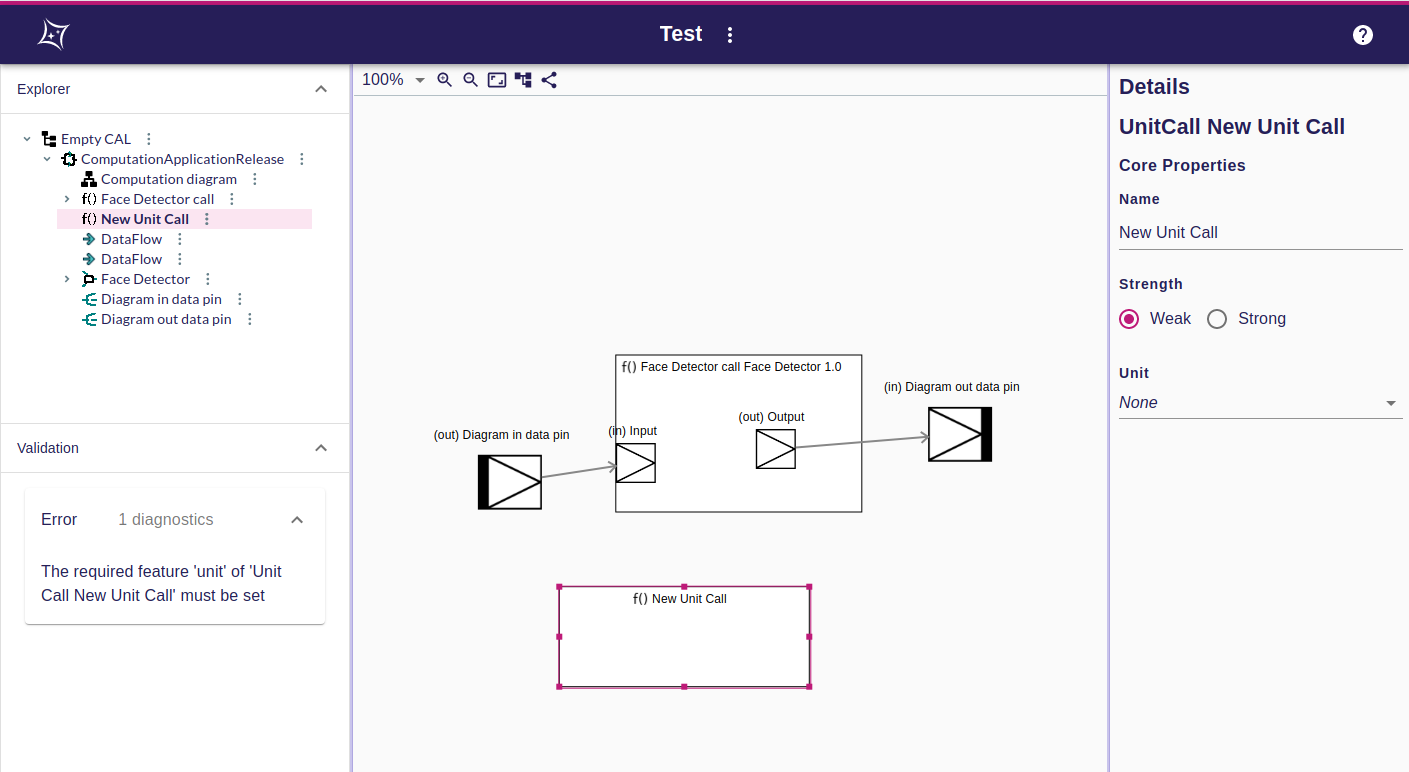
\includegraphics[width=0.95\linewidth]{./images/sirius-web-base-metamodel-model.png}
  \caption{Edycja modelu bazującego na przygotowanym metamodelu EMF w
  \emph{Sirius Web}.}\label{rys:sirius-web-base-metamodel-model}
\end{figure}
% \end{noindent}

W \emph{Sirius Web} można zdefiniować szablony modeli, które użytkownik może
wykorzystać chcąc stworzyć nowy model w projekcie. Umożliwia to prostszy
sposób na stworzenie chociażby pustego modelu, ponieważ przycisk tworzenia
modelu
na podstawie szablonu jest bardziej wyeksponowany w interfejsie użytkownika niż
przyciski tworzenia modelu z drzewa elementów projektu po lewej stronie.
Aby dodać nowy szablon należy dodać nowy opis \emph{stereotypu} w metodzie
\texttt{addStereotypeDescriptions} klasy
\texttt{StereotypeDescriptionRegistryConfigurer}. Kod odpowiedzialny za dodanie
nowego pustego szablonu modelu został przedstawiony
na~listingu~\ref{lst:empty-cal-model-template}. Interfejs użytkownika aplikacji
\emph{Sirius Web} wyświetlający nowo dodany szablon pustego modelu języka
\gls{CAL} został przedstawiony na
rysunku~\ref{rys:sirius-web-new-model-template}.

\begin{lstlisting}[float,
    floatplacement=!hb,
    language=Java,
    caption={Dodanie nowego pustego szablonu modelu języka CAL.},
    label={lst:empty-cal-model-template}]
    @Override
    public void addStereotypeDescriptions(IStereotypeDescriptionRegistry registry) {
        registry.add(new StereotypeDescription(
          UUID.nameUUIDFromBytes("empty_cal".getBytes()), //$NON-NLS-1$
          "Empty CAL", //$NON-NLS-1$
          this::getEmptyCALContent
        ));
    }

    private String getEmptyCALContent() {
        return this.stereotypeBuilder.getStereotypeBody(
          CALFactory.eINSTANCE.createComputationApplicationRelease()
        );
    }
\end{lstlisting}

% \begin{noindent}
\begin{figure}[!hb]
  \centering

  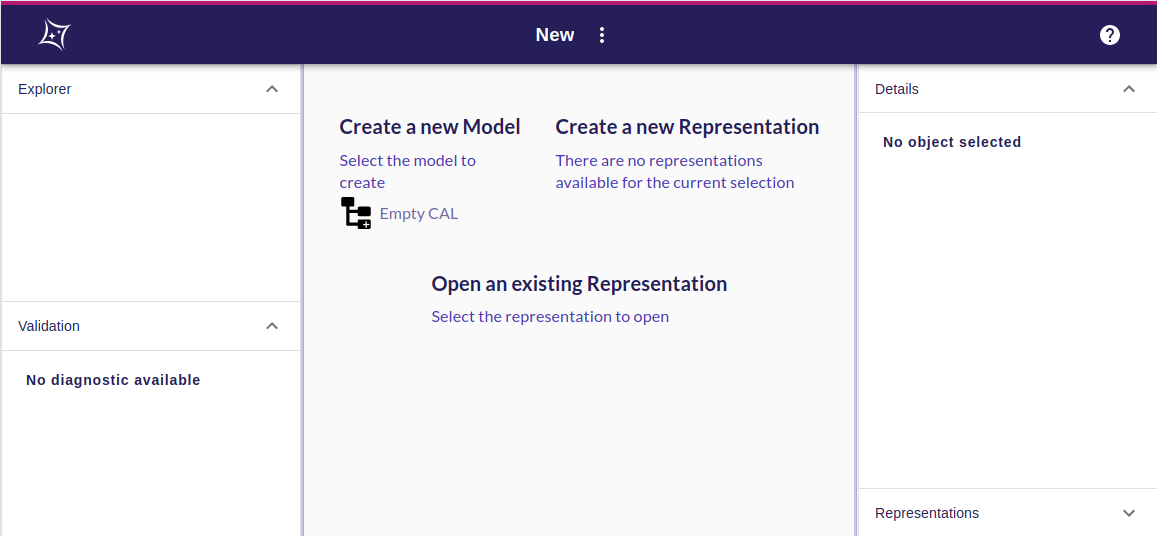
\includegraphics[width=0.95\linewidth]{./images/sirius-web-new-model-template.png}
  \caption{Szablon nowego pustego modelu języka
    \gls{CAL} w \emph{Sirius Web}.}\label{rys:sirius-web-new-model-template}
\end{figure}
% \end{noindent}

\subsection{Uruchamianie testów metamodelu za pomocą Maven}

W sekcji~\ref{sec:testy-metamodelu} opisano testy zmodyfikowanego zachowania
metamodelu EMF\@. Były one~uruchamianie w \emph{Sirius Desktop}. Z uwagi na
fakt, że
wygenerowany projekt z testami jest projektem typu \emph{Eclipse}, \emph{Apache
	Maven} nie ma możliwości wykonania tych testów podczas standardowego
polecenia
wykonania testów \lstinline{mvn test}.

Z pomocą przychodzi tutaj zestaw narzędzi \emph{Maven Tycho} wykorzystany do
połączenia metamodelu \gls{EMF} z \emph{Sirius Web}. Zawiera on rozszerzenie
\texttt{tycho-surefire-plugin}~\cite{maven-surefire-plugin-homepage}, które w
trakcie fazy wykonywania testów
integracyjnych w \emph{Maven} wykonuje również testy metamodelu zdefiniowane w
\emph{JUnit} i opisane w sekcji~\ref{sec:testy-metamodelu}.
Wykorzystanie go w pliku \texttt{pom.xml} projektu z testami (folder
\texttt{.tests}) przedstawione jest na
listingu~\ref{lst:pom-maven-surefire-plugin}. Należy w nim wskazać gdzie
znajduje się kod źródłowy testów oraz ścieżkę do pakietu z testami, a także
nazwę klasy grupującej wszystkie testy.

\begin{lstlisting}[float,
    floatplacement=!hb,
    language=XML,
    caption={Wykorzystanie rozszerzenia \emph{Maven Surefire} w
    \texttt{pom.xml} projektu z testami metamodelu.},
    label={lst:pom-maven-surefire-plugin}]
<build>
  <testSourceDirectory>${project.basedir}/src</testSourceDirectory>
  <plugins>
    <plugin>
      <groupId>org.eclipse.tycho</groupId>
      <artifactId>tycho-surefire-plugin</artifactId>
      <configuration>
        <testSuite>eu.balticlsc.model.CAL.tests</testSuite>
        <testClass>eu.balticlsc.model.CAL.tests.CALAllTests</testClass>
      </configuration>
      <version>2.5.0</version>
    </plugin>
  </plugins>
</build>
\end{lstlisting}

Po tak zmodyfikowanej konfiguracji
testy metamodelu \gls{EMF} w \emph{Maven} można uruchomić komendą
\lstinline{mvn verify}. Są one uruchamiane w fazie testów integracyjnych
(\texttt{verify}), a
więc po fazie budowania aplikacji (\texttt{package}). Powoduje to, że
uruchomienie testów metamodelu za~pomoca \emph{Maven} trwa dłużej (około
18 sekund), niż
wewnątrz \emph{Sirius Desktop} (mniej niż~1~sekunda), ponieważ projekt
najpierw musi zostać zbudowany. Dodatkowy narzut czasowy wprowadza także
komunikacja
\emph{Maven} z repozytorium \emph{Eclipse}, z którego pobierane są pakiety.
Niemniej jednak możliwość uruchomienia testów metamodelu w \emph{Maven} pozwala
na~uruchomienie ich z linii wiersza poleceń bez uruchamiania \emph{Sirius
	Desktop}, co przydaje się~w~środowisku serwerowym.

\section{Integracja przybornika BalticLSC w Sirius Web}

Opis problemu dodawania nowych \texttt{UnitCall} do diagramu --- trzeba
zdefiniować \texttt{ComputationUnitRelease} w diagramie.

Rozwiązanie (zaczerpnięte z edytora diagramów BalticLSC) --- przybornik
(toolbox).

Opis jak to zrobiono, od strony backendu jak i frontendu. Omówienie trudności w
modyfikacji interfejsu użytkownika Sirius Web (trzeba było skopiować kod
źródłowy niektórych komponentów z biblioteki \textit{Sirius Components} do kodu
aplikacji Sirius Web, ponieważ komponenty te nie umożliwiały modyfikacji
interfejsu i wstawiania do nich nowych elementów --- najlepiej dać zrzut ekranu
co można było łatwo zmienić, a co wymagało skopiowania kodu).

\section{Walidacja semantyczna modelu}

Informacja o informacjach diagnostycznych udostępnianych domyślnie przez Sirius
Web.

Brak uruchamiania reguł semantycznych zdefiniowanych w
metamodelu~\ref{sec:reguly-walidacyjne-metamodel}.

Opis dodanego rozwiązania (własne klasy Javowe które zwracają listę informacji
diagnostycznych, oraz strumieniowanie ich do przeglądarki wykorzystując
istniejące rozwiązanie do walidacji).

\section{Użycie edytora Sirius Web w BalticLSC}

Omówienie przygotowanego planu integracji.
